\subsection{\acs{laser} Focus Calculation}
\label{focus}
The figure \ref{fig:EmitterOptics} on page \ref{fig:EmitterOptics} gives a overview of the emitter optics. In order to diverge or focus the laser beam, it is possible to move the parabolic mirror up or down from the exact focus position. In this case, the divergent angle $\gamma$ needs to be calculated, which can be verified or optimized later on to obtain the desired footprint size. The calculation drawing is shown in figure \ref{fig:focus} on page \ref{fig:focus}.

\begin{figure}[ht!]
\centering
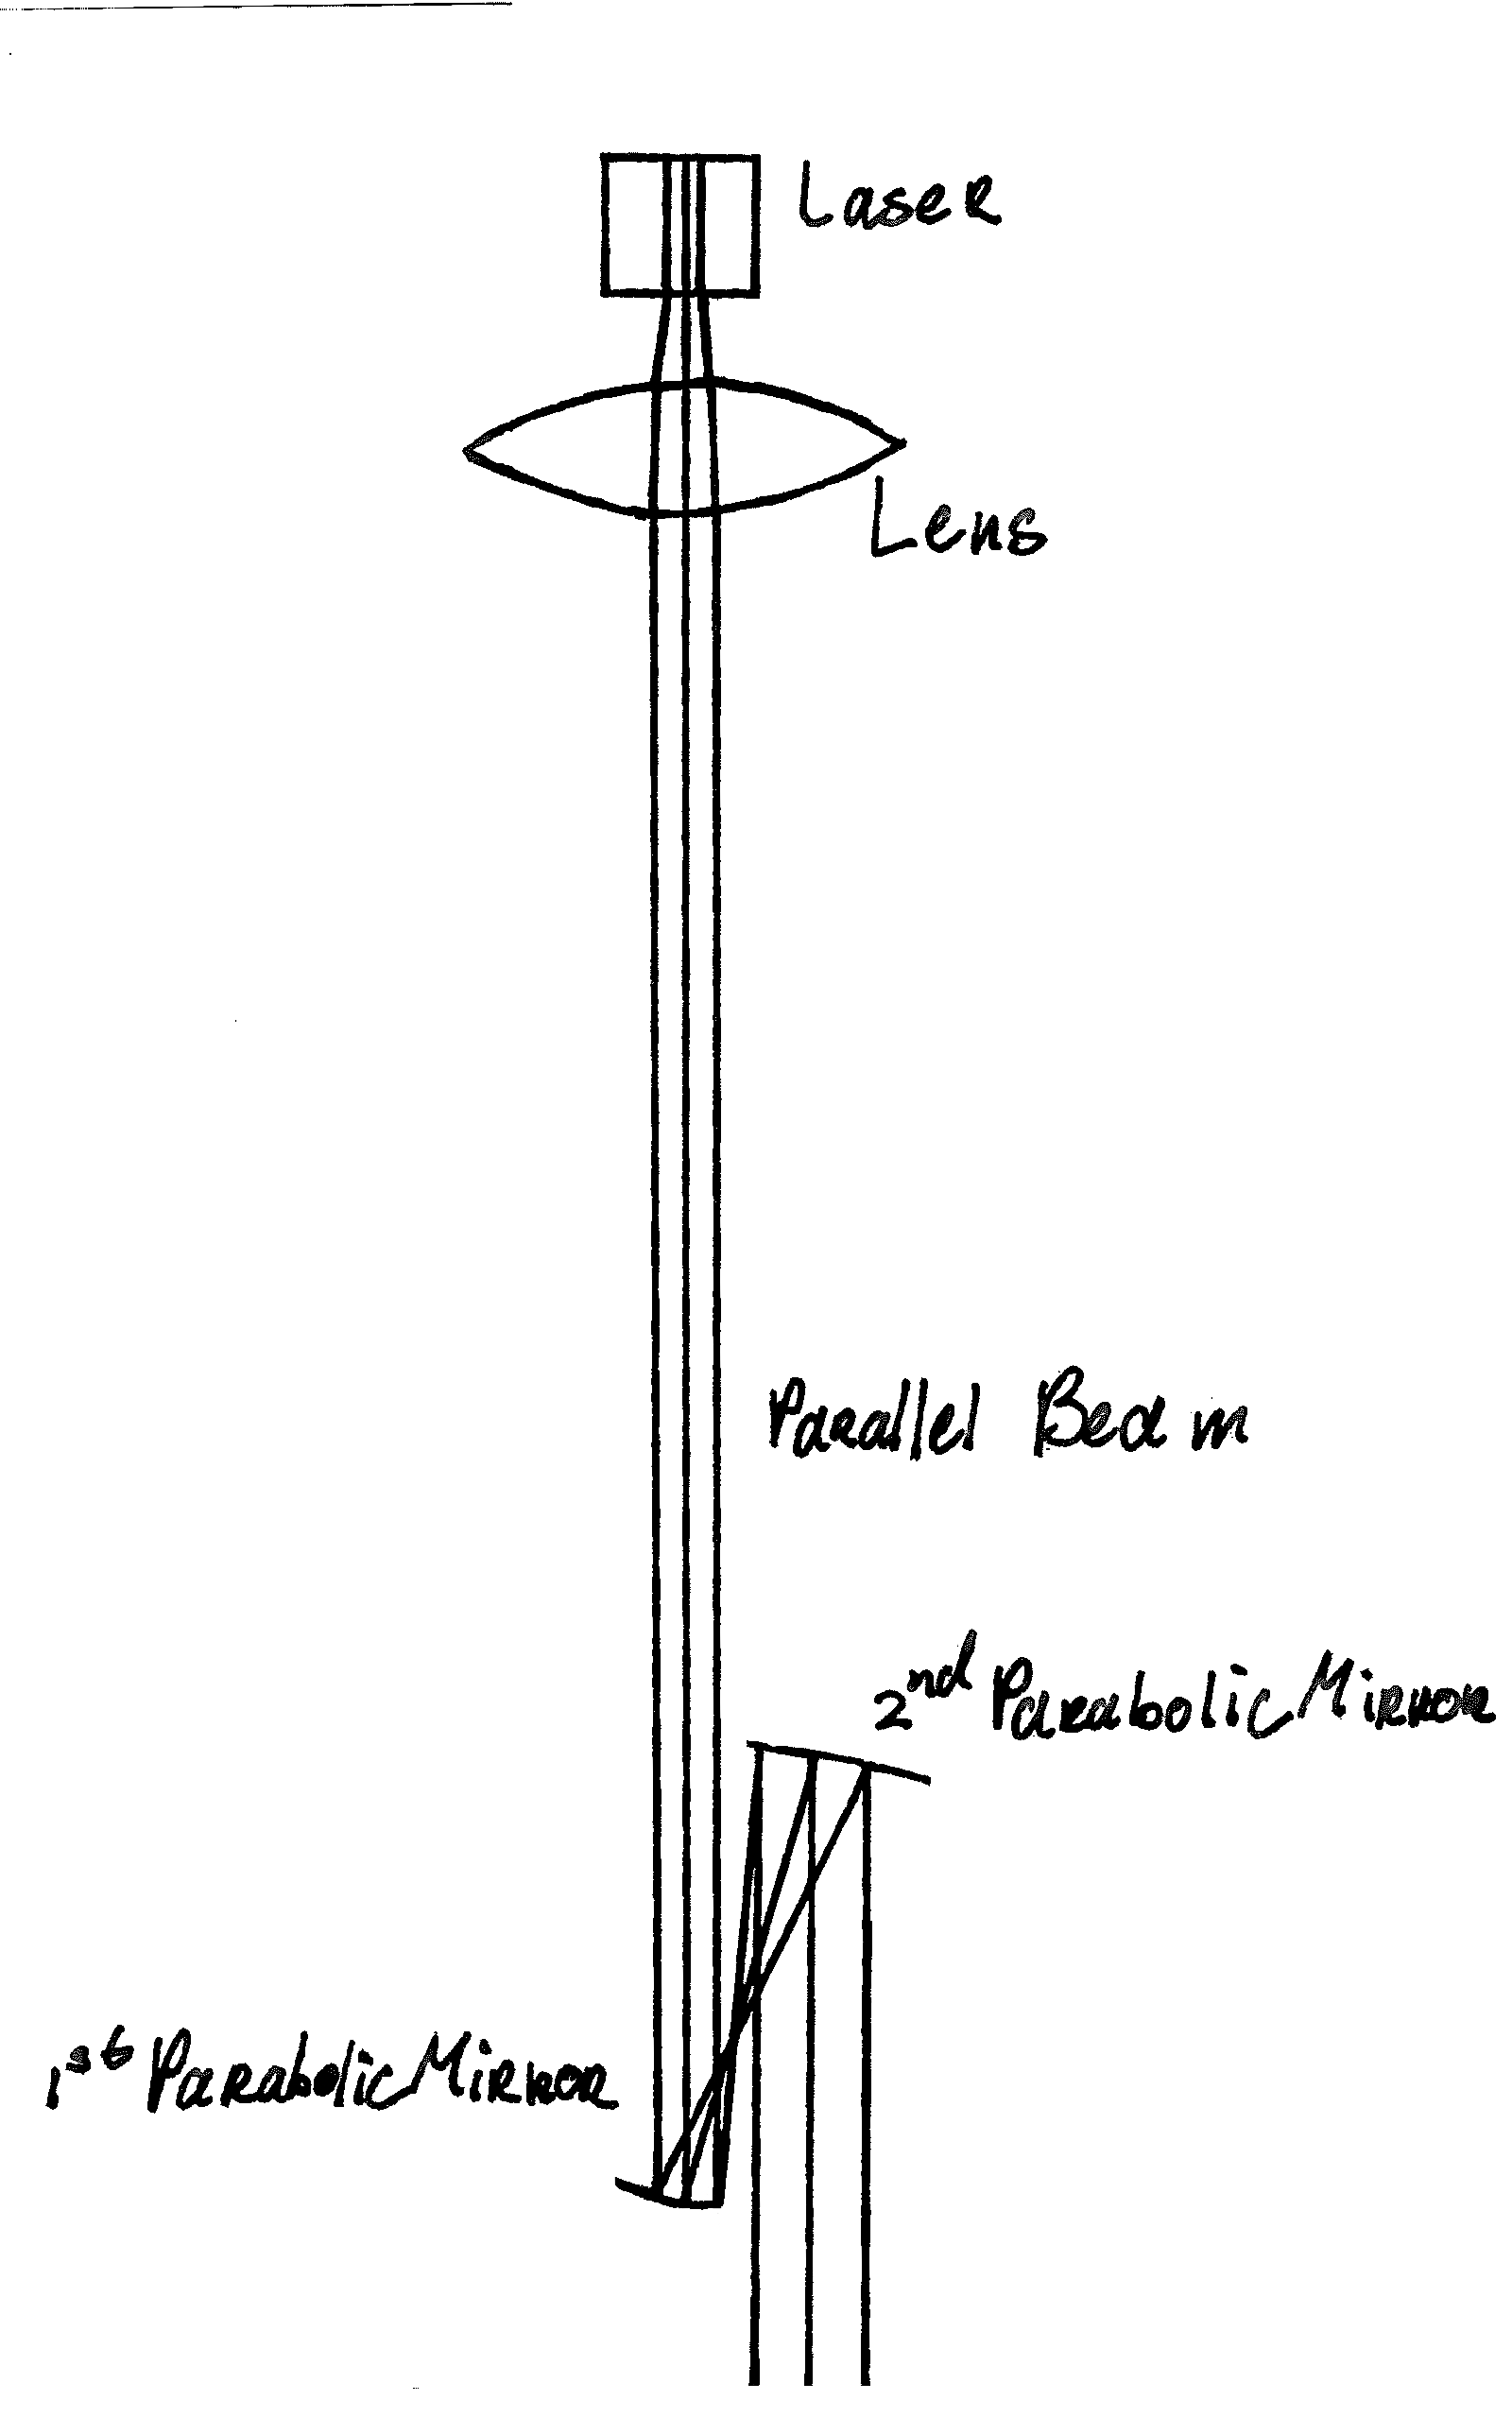
\includegraphics[scale = 0.8]{chapters/img/EmitterOptics.png}
\caption{Emitter optics drawing}
\label{fig:EmitterOptics}
\end{figure}

\begin{figure}[ht!]
\centering
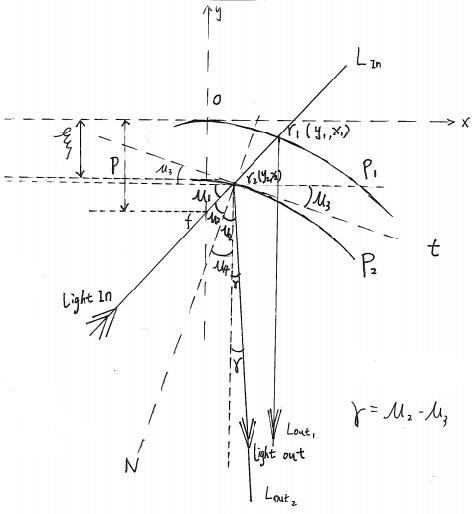
\includegraphics[scale = 1.2]{chapters/img/focus.png}
\caption{Focus calculation draft}
\label{fig:focus}
\end{figure}

In the figure \ref{fig:focus}, $p_{1}$ is the parabolic mirror positioned at the exact focus point f, and p is the distance between f and origin. $p_{2}$ is the parabolic mirror with the exact same shape but which is moved away from focus point with distance $\xi$. $L_{in}$ indicates the incoming light. $L_{out1}$ is the outcoming light due to $p_{1}$ and $L_{out2}$ is the outcoming light due to $p_{2}$. Meanwhile, $r_{1}(x_{1}, y_{1})$, $r_{2}(x_{2}, y_{2})$ are the reflected points due to $p_{1}$ and $p_{2}$. The purpose of this focusing calculation is to find the divergent angle $\gamma$ with respect to the design parameters p, $\xi$ and reflection point $r_{1}(x_{1}, y_{1})$. \cite{parabolic_wiki}Parabolic mirror $p_{1}$ has the equation \ref{p1}, and $p_{2}$ has the equation \ref{p2}. 
\begin{equation}
\label{p1}
y = -\frac{1}{4p}x^{2}
\end {equation}
\begin{equation}
\label{p2}
y = -\frac{1}{4p}x^{2}+\xi
\end {equation}
The equation \ref{Lin} for incoming light line $L_{in}$ can be obtained since $r_{1}(x_{1}, y_{1})$ is known in this case. 
\begin{equation}
\label{Lin}
y = \frac{y_{1}+p}{x_{1}}x-p
\end {equation}
Insert equation \ref{p2} into equation \ref{Lin}, $x_{2}$ of $r_{2}(x_{2}, y_{2})$ can be obtained as:
\begin{equation}
\label{x2}
x_{2} = \frac{-\frac{y_{1}+p}{x_{1}}+\sqrt{{\frac{y_{1}+p}{x_{1}}}^2-\frac{\xi-p}{p}}}{\frac{1}{2p}}
\end {equation}
Next step is to find the tangent line of $p_{2}$ at r2:
\begin{equation}
\label{miu3}
(\frac{dy}{dx})_{x_{2}} = -\frac{1}{2p}x_{2} = tan(\mu_{3}) \Rightarrow \mu_{3} = atan(-\frac{1}{2p}x_{2})
\end {equation}
In the figure, 't' is the tangent line at point $r_{2}$, and 'N' is the normal line perpendicular to the tangent line. The normal line 'N' is also the angle bisect, and $\mu_{2}$ is a half of the reflecting angle. From the drawing, these relations can be found:
\begin{equation}
\label{gamma}
\mu_{1}+\mu_{2}+\mu_{3} = 90^{\circ} = \mu_{1}+\mu_{2}+\mu_{4}
\Longrightarrow \gamma = \mu_{2} - \mu_{4} = \mu_{2} - \mu_{3} 
\end {equation}
To find $\mu_{2}$, $\mu_{1}$ need to be calculated. $\mu_{1}$ is the tangent angle of $L_{in}$ at $r_{1}$ or $r_{2}$:
\begin{equation}
\label{miu2}
(\frac{dy}{dx})_{x_{1},y_{1}} = \frac{y_{1}+p}{x_{1}} = tan(\mu{1})\Rightarrow \mu_{1} = atan(\frac{y_{1}+p}{x_{1}}) \Rightarrow \mu_{2} = 90deg - \mu_{1} - \mu_{3}
\end {equation}
Insert value of $\mu_{2}$ and $\mu_{3}$ to equation \ref{gamma}, so the divergent angle $\gamma = f(p, \xi, r_{1}(x_{1}, y_{1}))$ is obtained. Put these equations into Excel, and it is much easier to see how is $\gamma$ verified. For instance, give values for p=350[mm], $\xi$ = 5[mm] and $x_{1}$=5[mm], $\gamma$=0.01169[deg], which will give the footprint size of 102 meters. By adjusting the $\xi$, the mirror has a divergence of 20.4[m/mm] for the same p and $x_{1}$.